% Source-derived chapter 12: Possible configurations for Enriques surfaces
% Original source: no-enriques-surface-over-the-integers
\chapter{Possible configurations for Enriques surfaces}
\label{no-enriques-surface-over-the-integers-chapter-12}
\source{no-enriques-surface-over-the-integers}

\begin{remark}[Source section]
\label{no-enriques-surface-over-the-integers-chapter-12-source}
\source{no-enriques-surface-over-the-integers}
\source{no-enriques-surface-over-the-integers}
This chapter reproduces the corresponding section of the retrieved
LaTeX source, including its definitions, statements, examples, and
proofs. It has not yet been translated into Lean.
\notready
\end{remark}

% The source section title was: Possible configurations for Enriques surfaces
\mylabel{Possible configurations}

Let $Y$ be an Enriques surface over the prime field $k=\FF_2$ with constant Picard scheme. 
According to Theorem \ref{family with constant pic}, it admits at least one genus-one fibration.
Let us collect the information on   fibers we have gathered so far:

\begin{proposition}
\source{no-enriques-surface-over-the-integers}
\notready
\mylabel{possible configurations}
Let $\varphi:Y\ra\PP^1$ be a genus-one fibration.
Up to  automorphisms of the projective line,
the possible configurations of fibers over the the rational points $t=0,1,\infty$ are given by
the following table:
\begin{equation}
\label{first restriction}
\source{no-enriques-surface-over-the-integers}
\begin{array}[c]{@{}lll}
\toprule
\text{elliptic}		& 		& \text{quasielliptic}\\
\midrule
\II^*+E_4+\I_1		&		& \II^*+\II+\II\\
\II^*+E_2+\tI_1		&		& \III^*+\III+\II\\	 
\III^*+E_4+\I_2\\	 
\III^*+E_2+\tI_2\\
\III^*+E_4+E_4\\
\IV^*+E_3+\IV\\		 
\IV^*+E_5+\III\\
\midrule
\I_4^* +E_4+E_2		&		& \I_4^*+\II+\II\\
\I_1^*+E_5+\IV      &		& \I_2^*+\III+\III\\
\I_1^*+E_4+\I_4\\
\midrule
\III+E_4+\I_8\\
\bottomrule
\end{array}
\end{equation}
If moreover the Enriques surface $Y$ is non-exceptional, the following holds:
\begin{enumerate}
\item
Each fiber  with Kodaira symbol  $\IV$, $\IV^*$,   $\II^*$, $\I_1^*$ is multiple.
\item
If there is a simple fiber with Kodaira symbol $\III^*$, the fibration is elliptic, and the configuration
of fibers over rational points is $\III^*+E_4+E_4$.
\item
For each multiple fiber $\varphi^{-1}(a)$ with Kodaira symbol $\IV^*$, $\III^*$ or $\II^*$, there is  no $(-2)$-curve
$R\subset Y$ with intersection number  $\varphi^\inv_\ind(a)\cdot R=1$.
\end{enumerate}
\end{proposition}

\proof
The main task is to verify the table.
Let $\bar{a}:\Spec(\Omega)\ra \PP^1$ be a geometric point, with image $a\in \PP^1$.
If this image point is non-rational, the geometric fiber $Y_\ba$ is irreducible, 
according to Theorem \ref{geometric and schematic fiber}.
In any case,  the map $\Gamma(Y_\ba)\ra\Gamma(Y_a)$ between dual graphs is a graph isomorphism.
Moreover, the Kodaira symbol $\I_0^*$ is impossible, according to Proposition \ref{canonical type rational points}.
In particular, $Y_a$ and $Y_\ba$ have the same number of irreducible components. Write $r_a\geq 1$ for this number.
Then we have the inequality $2+\sum (r_a-1)\leq \rho(Y)=10$, and thus  $r_0+r_1+r_\infty\leq 11$.

Suppose first that the fibration is quasielliptic.  Since the Picard group $\Pic^0(Y_F)$ for the generic fiber  
is annihilated by $p=2$, we actually have  $r_0+r_1+r_\infty=11$. The possible Kodaira symbols
and
the corresponding number of irreducible components  are as follows (\cite{Cossec; Dolgachev 1989}, Theorems 5.7.4--5.7.6):
$$
\begin{array}{lllllll}
\toprule
\text{Kodaira symbol}			& \II	& \III	& \I_2^*	& \III^*	& \II^*	& \I_4^*\\
\midrule
\text{number of irr.\ comp.}	& 1		& 2		& 7			& 8			& 9		& 9\\
\bottomrule
\end{array}
$$
Since $9+1+1=8+2+1=7+2+2=11$ are the only possible solutions, the second column of table \eqref{first restriction} follows.

Now suppose that $\varphi:Y\ra\PP^1$ is elliptic, and consider the resulting jacobian fibration $\phi:J\ra\PP^1$.
Then the smooth proper surface $J$ is geometrically rational (Proposition \ref{jacobian geometrically rational}), 
with constant Picard scheme (Theorem \ref{jacobian constant pic}).
As above, the geometric fibers $J_\ba$ are irreducible if $a\in \PP^1$ is non-rational,
and in any case $\Gamma(J_\ba)\ra\Gamma(J_a)$ is a graph isomorphism.
According to Theorems \ref{classification non-zero j} and \ref{classification zero j}, 
the first column of table \eqref{first restriction} gives the possible configurations
of singular fibers over the  rational points for $\phi:J\ra\PP^1$. 
By Proposition \ref{same symbols} the fibers $Y_\ba$ and $J_\ba$ have the same Kodaira symbols. 
Moreover, we  actually have $J_a\simeq Y_a$ if the fiber $Y_a$ is simple. In particular, this holds for all semistable
fibers. According to Proposition \ref{reduction isomorphic}, we also have $J_a\simeq (Y_a)_\red$ provided that $Y_a$ is multiple 
with smooth reduction. In turn, the first column of table \eqref{first restriction} indeed describes the configuration of
degenerate fibers for $\varphi:Y\ra\PP^1$.

Now suppose that $Y$ is non-exceptional. If $\varphi:Y\ra\PP^1$ is elliptic 
having some $\varphi^{-1}(a)$ with Kodaira symbol $\IV,\IV^*,\II^*,\I_1^*$ there must   be 
some $\varphi^\inv_\ind(b)$ that is supersingular or semistable, in light of  the table,
so $\varphi^{-1}(a)$ is multiple by Lemma \ref{multiple for p=2}.
If $\varphi:Y\ra\PP^1$ is quasielliptic, fibers with Kodaira symbol $\II^*$ are multiple 
according to    Proposition \ref{properties non-exceptional}. This establishes (i).

Next assume that $\varphi^{-1}(a)$ is simple with Kodaira symbol $\III^*$.
Again by Proposition \ref{properties non-exceptional} the fibration must be elliptic. By the table, the configuration
of fibers over rational points is $\III^*+E_4+\I_2$ or  $\III^*+E_2+\tI_2$ or $\III^*+E_4+E_4$.
The former are impossible by Lemma \ref{multiple for p=2}, which gives (ii).
Finally, assertion (iii) is a consequence of    Proposition \ref{properties non-exceptional}.
\qed

\medskip
Starting from the above information, we rule out step by step each possible Kodaira symbol, 
mostly from combinatorial considerations.  In this section, we will reduce
from fifteen to eight possible configurations for $\varphi:Y\ra\PP^1$.

\begin{proposition}
\source{no-enriques-surface-over-the-integers}
\notready
\mylabel{no I8}
Assumption as in Proposition \ref{possible configurations}.
Then there are no fibers with   Kodaira symbol $\I_8$. 
\end{proposition}

\proof
Seeking a contradiction, we assume that $\varphi^{-1}(\infty)$ has Kodaira symbol $\I_8$, and $\varphi^{-1}(0)$ has symbol $\III$.
Then   the configuration of reducible fibers has dual graph:
% \begin{equation*}
% % dual graph III+I8
% \begin{gathered}
% \begin{tikzpicture}
% [node distance=1cm, font=\small]
% \tikzstyle{vertex}=[circle, draw, fill=white, inner sep=0mm, minimum size=1.5ex]
% \node[vertex]	(C0)  	at (1,0) 	[label=above:{$C_0$}] 		{};
% \node[vertex]	(C1)			[below left of=C0, label=left:{$C_1$}]	{};
% \node[vertex]	(C2)			[below of=C1, label=left:{$C_2$}]	{};
% \node[vertex]	(C3)			[below right of=C2, label=below:{$C_3$}]	{};
% \node[vertex]	(C4)			[right of=C3, label=below:{$C_4$}]	{};
% \node[vertex]	(C5)			[above right of=C4, label=right:{$C_5$}]	{};
% \node[vertex]	(C6)			[above of=C5, label=right:{$C_6$}]	{};
% \node[vertex]	(C7)			[above left of=C6, label=above:{$C_7$}]	{};
%  
% \node[vertex]	(D0)			[above left of=C1, ,  xshift=-4em, yshift=-1em, label=above:{$D_0$}]	{};
% \node[vertex]	(D1)			[below left of=C2,  xshift=-4em, yshift=+1em, label=below:{$D_1$}]	{};
%  
% \draw[thick] (C0)--(C1)--(C2)--(C3)--(C4)--(C5)--(C6)--(C7)--(C0);
% \draw[thick,double] (D0)--(D1);
% \end{tikzpicture}
% \end{gathered}
% \end{equation*}
\begin{equation*}
% dual graph III+I8
\begin{gathered}
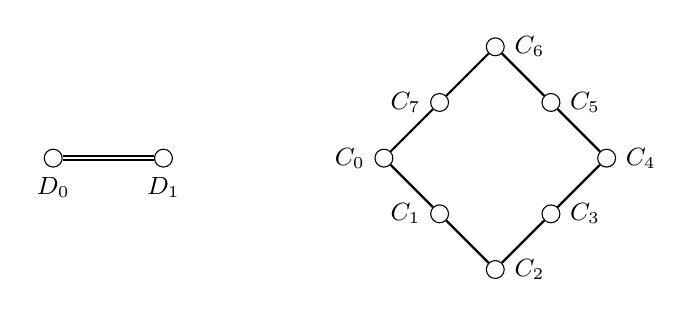
\begin{tikzpicture}
[node distance=1cm, font=\small]
\tikzstyle{vertex}=[circle, draw, fill=white, inner sep=0mm, minimum size=1.5ex]
\node[vertex]	(C0)  	at (0,0)[label=left:{$C_0$}] 		{};
\node[vertex]	(C1)			[below right of=C0, label=left:{$C_1$}]	{};
\node[vertex]	(C2)			[below right of=C1, label=right:{$C_2$}]	{};
\node[vertex]	(C3)			[above right of=C2, label=right:{$C_3$}]	{};
\node[vertex]	(C4)			[above right of=C3, label=right:{$C_4$}]	{};
\node[vertex]	(C5)			[above left of=C4, label=right:{$C_5$}]	{};
\node[vertex]	(C6)			[above left of=C5, label=right:{$C_6$}]	{};
\node[vertex]	(C7)			[below left of=C6, label=left:{$C_7$}]	{};
 
\node[]         (E)             [left of=C0,  xshift=-0.4cm,  label=below:{$$}]	{};
\node[vertex]	(D1)			[left of=E,  xshift=-0.4cm,  label=below:{$D_1$}]	{};
\node[vertex]	(D0)			[left of=D1,  xshift=-0.4cm, label=below:{$D_0$}]	{};
 
\draw[thick] (C0)--(C1)--(C2)--(C3)--(C4)--(C5)--(C6)--(C7)--(C0);
\draw[thick,double] (D0)--(D1);
\end{tikzpicture}
\end{gathered}
\end{equation*}
\emph{Here the double edge indicates that the   scheme $D_0\cap D_1$ has length two}.
The semistable fiber $\varphi^{-1}(\infty)$  is simple whereas the unstable fiber $\varphi^{-1}(0)$  is multiple.
Moreover,  there is a genus-one fibration $\psi:Y\ra\PP^1$ so that the multiple fibers $2F$ have  
$F\cdot \varphi^\inv_\ind(0)=1$. 
After renumeration, we may assume   $(F\cdot D_1)=1$, hence $D_0$ is vertical with respect to $\psi$.
Without restriction, we may assume that $\psi^\inv(\infty)$ is simple, whereas the $\psi$-fibers over $a=0,1$ are multiple.
Write $\psi^\inv_\ind(0)=\sum_{i=0}^r m_i \Theta_i$. After renumeration, we may assume $(D_1\cdot \Theta_0)>0$.
From
$$
1=\varphi^\inv_\ind(0)\cdot\psi^\inv_\ind(0) = D_1\cdot \sum_{i=0}^rm_i\Theta_i = m_0(D_1\cdot\Theta_0) + \sum_{i=1}^r m_i(D_1\cdot\Theta_i)
$$
we see that $(D_1\cdot\Theta_0)=m_0=1$, and that the curve $\Theta_1+\ldots+\Theta_r$  is disjoint from $D_1$.
Furthermore, $D_0$ does not belong to $\psi^\inv(0)$, because   $D_0=\Theta_j$ gives the contradiction
$$
1=\varphi^\inv_\ind(0)\cdot\psi^\inv_\ind(0) = D_1\cdot\psi^\inv_\ind(0)\geq D_1\cdot m_j\Theta_j\geq 2m_j\geq 2.
$$
Consequently $\Theta_1+\ldots+\Theta_r\subset\varphi^{-1}(\infty)$.
From $m_0=1$ we infer that  $\Theta_1+\ldots+\Theta_r$ is connected, hence is a chain. So the multiple fiber $\psi^\inv_\ind(0)$ is either
ordinary or has Kodaira symbol $\II$, $\III$ or $\IV$.
The same analysis applies to the other multiple fiber $\psi^\inv_\ind(1)$.
From Proposition \ref{possible configurations}, we see that the possible Kodaira symbols for  the simple fiber $\psi^\inv(\infty)$
are $\I_8$ or $\II^*, \III^*, \I_4^*, \I_2^*$.

To proceed write  $\psi^\inv(\infty)=\sum_{i=0}^s n_i\Upsilon_i$. Then $s\geq 6$ and  $(\Upsilon_i\cdot\Upsilon_j)\leq 1$. After renumeration $\Upsilon_0=D_0$. From
$$
2=\varphi^\inv_\ind(0)\cdot\psi^\inv(\infty) = D_1\cdot\sum_{i=0}^s n_i\Upsilon_i = 2n_0 + \sum_{i=1}^s n_i(D_1\cdot\Upsilon_i)
$$
we infer $n_0=1$, and that $\Upsilon_1+\ldots+\Upsilon_s$ is disjoint from $D_1$.
Seeking a contradiction, we now assume that $\psi^{-1}(\infty)$ is additive. By inspection, one sees that  $\Upsilon_0$ has exactly one neighbor in the dual graph,
say $\Upsilon_1$, and  that $\Upsilon=\Upsilon_2+\ldots+\Upsilon_s$ is not a disjoint union of chains.
Moreover, $\Upsilon$ is disjoint from $\varphi^{-1}(0)$, hence must be strictly 
contained in $\varphi^\inv(\infty)$. The latter is multiplicative, and it follows that $\Upsilon$ is a union of chains, contradiction.
We conclude that $\psi^\inv(\infty)$ has Kodaira symbol $\I_8$.
% The component $\Upsilon_0$ has $t\leq 2$ neighbors in the dual graph, say $\Upsilon_1,\ldots,\Upsilon_t$.
% In turn, $\Upsilon=\Upsilon_{t+1}+\ldots+\Upsilon_s$ is disjoint from $\varphi^{-1}(0)$, hence must be contained in $\varphi^\inv(\infty)$.
% So the dual graph for $\Upsilon$ is a union of chains, and we conclude that $\psi^\inv(\infty)$ has Kodaira symbol $\I_8$.

Summing up, the configuration of rational fibers for $\psi$
must be $\III+E_4+\I_8$, according to the   table in Proposition \ref{possible configurations}.
Without restriction we may assume that $\psi^{-1}_\ind(0)=\Theta_0+\Theta_1$ is reducible.
We saw above that $\Theta_1$ belongs to $\varphi^\inv(\infty)$, so after renumeration $\Theta_1=C_0$.
To simplify notation set $E=\Theta_0$, such that
$\psi^\inv_\ind(0)=E+C_0$   with $(E\cdot D_1)=1$ and $(E\cdot C_0)=2$. 
It follows that  $D_0$ and $C_2+\ldots+C_6$ belong  to $\psi^\inv(\infty)$. Let $E_1,E_7$ be the additional components.
The dual graph for our curves takes the following form:
\begin{equation*}
% dual graph III+I8
\begin{gathered}
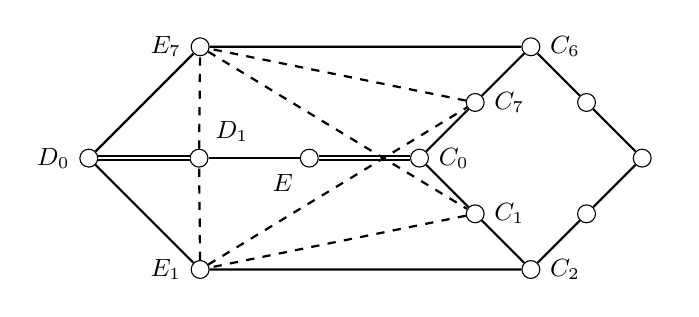
\begin{tikzpicture}
[node distance=1cm, font=\small]
\tikzstyle{vertex}=[circle, draw, fill=white, inner sep=0mm, minimum size=1.5ex]
\node[vertex]	(C0)  	at (0,0)[label=right:{$C_0$}] 		{};
\node[vertex]	(C1)			[below right of=C0, label=right:{$C_1$}]	{};
\node[vertex]	(C2)			[below right of=C1, label=right:{$C_2$}]	{};
\node[vertex]	(C3)			[above right of=C2, label=right:{}]	{};
\node[vertex]	(C4)			[above right of=C3, label=right:{}]	{};
\node[vertex]	(C5)			[above left of=C4, label=right:{}]	{};
\node[vertex]	(C6)			[above left of=C5, label=right:{$C_6$}]	{};
\node[vertex]	(C7)			[below left of=C6, label=right:{$C_7$}]	{};
 
\node[vertex]   (E)             [left of=C0,  xshift=-0.4cm,  label=below left:{$E$}]	{};
\node[vertex]	(D1)			[left of=E,  xshift=-0.4cm,  label=above right:{$D_1$}]	{};
\node[vertex]	(D0)			[left of=D1,  xshift=-0.4cm, label=left:{$D_0$}]	{};

\node[vertex]   (E7)            [left of=C6,  xshift=-3.2cm,  label=left:{$E_7$}]	{};
\node[vertex]   (E1)            [left of=C2,  xshift=-3.2cm,  label=left:{$E_1$}]	{};

\draw[thick] (C0)--(C1)--(C2)--(C3)--(C4)--(C5)--(C6)--(C7)--(C0);
\draw[thick,double] (D0)--(D1);
\draw[thick,double] (E)--(C0);
\draw[thick] (E)--(D1);
\draw[thick] (C2)--(E1)--(D0)--(E7)--(C6);
\draw[thick,dashed] (C7)--(E7)--(C1);
\draw[thick,dashed] (C1)--(E1)--(C7);
\draw[thick,dashed] (E1)--(D1)--(E7);
\end{tikzpicture}
\end{gathered}
\end{equation*}
\emph{Here the dashed edges indicate potential intersections}.
Using
$$
2=(D_0+D_1) \cdot\sum \psi^\inv(\infty) = (D_0+D_1)\cdot(E_1+E_7) = 1+1 + D_1\cdot(E_1+E_7)
$$
we conclude that $D_1$ is actually disjoint from $E_1\cup E_7$. Then
$$
2=2(D_0+D_1)\cdot E_1 = (C_0+\ldots+C_7)\cdot E_1 = (C_1+C_7)\cdot E_1 +1
$$
ensures that either $(E_1\cdot C_1)=1$, $(E_1\cdot C_7)=0$ or $(E_1\cdot C_7)=1$, $(E_1\cdot C_1)=0$.
In the former case we get a curve    $E_1+C_2+C_1$ of canonical type $\I_3$, in the letter 
$E_1+C_2+\ldots+C_7$ of canonical type $\I_7$, contradiction.
\qed

\medskip
For the next observation it is crucial to  exclude exceptional Enriques surfaces.

\begin{proposition}
\source{no-enriques-surface-over-the-integers}
\notready
\mylabel{no II*, IV*, IV}
Assumption as in Proposition \ref{possible configurations}. Assume  $Y$ is non-exceptional. 
Then there are no fibers with Kodaira symbol $\II^*$, $\IV^*$ or  $\IV$. Furthermore, there are no multiple fiber
with Kodaira symbol $\I_4^*$.
\end{proposition}

\proof
According to Proposition \ref{possible configurations}, all fibers with Kodaira symbol $\II^*$, $\IV^*$, $\IV$ are multiple.
Seeking a contradiction, we thus assume that $\varphi^{-1}(\infty)$ is a multiple with  Kodaira symbol $\II^*$, $\IV^*$, $\IV$ 
or  $\I_4^*$.
 
By  Proposition \ref{properties non-exceptional}, there is another genus-one fibrations $\psi:Y\ra\PP^1$ 
such that  $\varphi^{-1}(\infty)\cdot \psi^{-1}(\infty)=4$.
Without restriction, we may assume that $\psi^{-1}(\infty)$ is the   fiber  having
the maximal number of irreducible components.
Let  $2F$  a  multiple fiber  for $\psi$, such that  $F\cdot \varphi_\ind^{-1}(\infty)=1$.
 
We first treat the case   that  
$\varphi^{-1}(\infty)$ is multiple with Kodaira symbol $\II^*$. With enumeration as in the Bourbaki tables
\cite{LIE 4-6}, the dual graph for such a  fiber is:
\begin{equation*}
% dual graph II*
\begin{gathered}
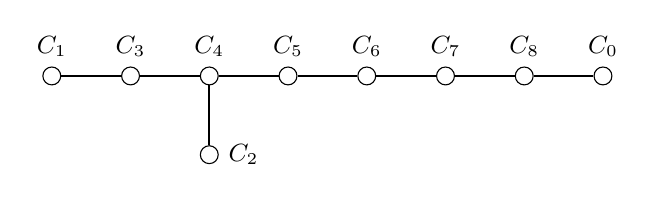
\begin{tikzpicture}
[node distance=1cm, font=\small]
\tikzstyle{vertex}=[circle, draw, fill=white, inner sep=0mm, minimum size=1.5ex]
\node[vertex]	(C1)  	at (1,0) 	[label=above:{$C_1$}] {};
\node[vertex]	(C3)			[right of=C1,  label=above:{$C_3$}]	{};
\node[vertex]	(C4)			[right of=C3,  label=above:{$C_4$}]	{};
\node[vertex]	(C2)			[below of=C4,  label=right:{$C_2$}]	{};
\node[vertex]	(C5)			[right of=C4,  label=above:{$C_5$}]	{};
\node[vertex]	(C6)			[right of=C5,  label=above:{$C_6$}]	{};
\node[vertex]	(C7)			[right of=C6,  label=above:{$C_7$}]	{};
\node[vertex]	(C8)			[right of=C7,  label=above:{$C_8$}]	{};
\node[vertex]	(C0)			[right of=C8,  label=above:{$C_0$}]	{};

\draw[thick]    (C1)--(C3)--(C4)-- (C5)--(C6)--(C7)--(C8)--(C0);
\draw[thick]    (C2)--(C4);
\end{tikzpicture}
\end{gathered}
\end{equation*}
We also denote this dual graph by $T_{2,3,6}$. \emph{In general, the symbol $T_{l,m,n}$ refers to a star-shaped graph
with three terminal chains of length $l,m,n$, where the central vertex belongs to each of the terminal chains}.

We have $\varphi^{-1}_\ind(\infty)=C_0+2C_1+3C_2+\ldots +2C_8$, and $C_0$ is indeed the only component  with multiplicity $m=1$.
Thus  $(C_0\cdot F)=1$.  
In turn, the connected curve $C_1+\ldots+C_8$ has dual graph $T_{2,3,5}$ and is necessarily contained in
the fiber $\psi^{-1}(\infty)$, which therefore must have Kodaira symbol $\II^*$. This is multiple by 
Proposition \ref{possible configurations}.
Let $R\subset\psi^{-1}(\infty)$ be the additional component, with $(R\cdot C_8)=1$.
Then 
$$
1=\varphi^{-1}_\ind(\infty)\cdot\psi^{-1}_\ind(\infty) =  \varphi^{-1}_\ind(\infty)\cdot R= (C_0+2C_8)\cdot R\geq 2(C_8\cdot R)=2,
$$
contradiction. Summing up, there are no fibers with Kodaira symbol $\II^*$.

Suppose next that $\varphi^{-1}(\infty)$ is multiple with Kodaira symbol $\I_4^*$.
The dual graph is:
\begin{equation*}
% dual graph I4*
\begin{gathered}
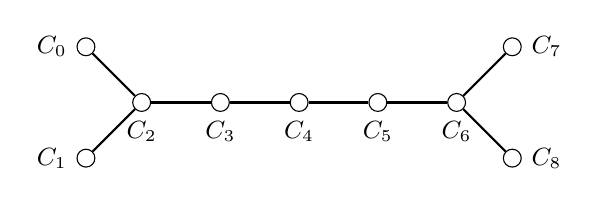
\begin{tikzpicture}
[node distance=1cm, font=\small]

\tikzstyle{vertex}=[circle, draw, fill=white, inner sep=0mm, minimum size=1.5ex]
\node[vertex]	(C2)  	at (1,0) 	[label=below:{$C_2$}] 		{};
\node[vertex]	(C3)			[right of=C2, label=below:{$C_3$}]	{};
\node[vertex]	(C4)			[right of=C3, label=below:{$C_4$}]	{};
\node[vertex]	(C5)			[right of=C4, label=below:{$C_5$}]	{};
\node[vertex]	(C6)			[right of=C5, label=below:{$C_6$}]	{};

\node[vertex]	(C7)			[above right of=C6, label=right:{$C_7$}]	{};
\node[vertex]	(C8)			[below right of=C6, label=right:{$C_8$}]	{};
\node[vertex]	(C0)			[above left  of=C2, label=left :{$C_0$}]	{};
\node[vertex]	(C1)			[below left  of=C2, label=left :{$C_1$}]	{};

\draw [thick] (C2)--(C3)--(C4)--(C5)--(C6);
\draw [thick] (C0)--(C2)--(C1);
\draw [thick] (C7)--(C6)--(C8);
\end{tikzpicture}
\end{gathered}
\end{equation*}
Now $\varphi^{-1}_\ind(\infty) = C_0+C_1+2(C_2+\ldots+C_6)+C_7+C_8$.
After renumeration, we may assume $(F\cdot C_0)=1$.
In turn, the connected curve $C_1+\ldots+C_8$ has dual graph $T_{2,2,6}$, and is necessarily contained
in $\psi^{-1}(\infty)$. This must have Kodaira symbol $\I_4^*$, as we already ruled out the symbol $\II^*$.
Let $R\subset \psi^{-1}(\infty)$ be the additional component, with $(R\cdot C_2)=1$.
We then have
$$
2\geq \varphi^{-1}_\ind(\infty)\cdot \psi^{-1}_\ind(\infty) = \varphi^{-1}_\ind(\infty)\cdot R = (C_0+2C_2)\cdot R=(C_0\cdot R)+2.
$$
Consequently $C_0\cap R=\varnothing$. In turn, $C_0+\ldots+C_3+R$ supports a curve of canonical type $\I_0^*$, 
in contradiction to Proposition \ref{possible configurations}.
So there are no multiple fibers with Kodaira symbol $\I_4^*$.

Suppose next that $\varphi^{-1}(\infty)$ is multiple with Kodaira symbol $\IV^*$.
The dual graph for $\varphi^{-1}(\infty)$ is:
\begin{equation*}
% dual graph IV*
\begin{gathered}
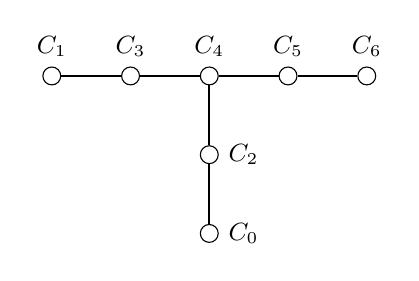
\begin{tikzpicture}
[node distance=1cm, font=\small]
\tikzstyle{vertex}=[circle, draw, fill=white, inner sep=0mm, minimum size=1.5ex]
\node[vertex]	(C1)  	at (1,0) 	[label=above:{$C_1$}] {};
\node[vertex]	(C3)			[right of=C1,  label=above:{$C_3$}]	{};
\node[vertex]	(C4)			[right of=C3,  label=above:{$C_4$}]	{};
\node[vertex]	(C2)			[below of=C4,  label=right:{$C_2$}]	{};
\node[vertex]	(C5)			[right of=C4,  label=above:{$C_5$}]	{};
\node[vertex]	(C6)			[right of=C5,  label=above:{$C_6$}]	{};
 \node[vertex]	(C0)			[below of=C2,  label=right:{$C_0$}]	{};

\draw[thick]    (C1)--(C3)--(C4)-- (C5)--(C6);
\draw[thick]    (C4)--(C2)--(C0);
\end{tikzpicture}
\end{gathered}
\end{equation*}
Now $\varphi^\inv_\ind(\infty)=(C_0+C_1+C_6)+2(C_2+C_3+C_5)+ 3C_4$.
After renumeration  we have $(F\cdot C_0)=1$. In turn, the connected curve $C_1+\ldots+C_6$ has dual graph $T_{2,3,3}$
and must be contained in $\psi^{-1}(\infty)$. 
Now recall that we already established that $\II^*$ does not appear in any genus-one fibration on $Y$.
Consequently, the only possible Kodaira symbols for
the fiber $\psi^{-1}(\infty)$ are $\IV^*$ and $\III^*$. 
In the former case, the fiber is multiple  by Proposition \ref{possible configurations},
and we write  $R\subset\psi^{-1}(\infty)$ for the additional component. 
Then $1=\varphi^{-1}_\ind(\infty)\cdot\psi^{-1}_\ind(\infty) = (C_0+2C_2)\cdot R\geq 2$, contradiction.
So the fiber $\psi^{-1}(\infty)$ has Kodaira symbol $\III^*$.
Let $R,R'\subset\psi^{-1}(\infty)$ be the two additional components, say with
$(R\cdot C_1)=(R'\cdot C_6)=1$. Then
$$
2\geq \varphi^{-1}_\ind(\infty)\cdot\psi^{-1}_\ind(\infty)  = (C_0+C_1+C_6)\cdot (R+R')= (C_0\cdot R) + (C_0\cdot R')+2.
$$
It follows that $\psi^{-1}(\infty)$ is simple. In light of Proposition \ref{possible configurations}, 
the configuration of fibers over the rational points  for $\psi:Y\ra\PP^1$
is $\III^*+E_4+E_4$. In turn, each $(-2)$-curve $C\subset Y$ intersects the fiber $\psi^{-1}(\infty)$.
By Proposition \ref{possible configurations}, 
we may assume that $\varphi^{-1}(0)=2(C_0'+\ldots+C_{r-1}')$ is multiple with  Kodaira symbol $\III$ or $\IV$
with respective integers $r=2$ or $r=3$.
Obviously  $C_0,\ldots,C_6$ are disjoint from  $\varphi^{-1}(0)$.
In turn, $R\cup R'$ intersects each component $C'_i\subset\varphi^\inv(0)$.
Moreover, $R$ is not contained in $\varphi^{-1}(0)$, because 
$R\cdot\varphi^{-1}(0) = R\cdot \varphi^{-1}(\infty)\geq 1$, and likewise for $R'$.
So $2=\varphi^{-1}_\ind(0) \cdot \psi^{-1}(\infty) $ equals
$$
(C_0'+\ldots+C'_{r-1})\cdot \psi^{-1}(\infty) = (C_0'+\ldots+C'_{r-1})\cdot(R+R') \geq r\geq 2.
$$
Thus we have equality at each step, hence $r=2$, and the fiber $\varphi^{-1}(0)$ has Kodaira symbol $\III$.
If $R,R'$ intersect the same component of $\varphi^{-1}(0)$, say $C'_0$, the curve $C_3+\ldots+C_6+R'+C'_0+R+ C_1$ is
a curve of canonical type $\I_8$, in contradiction to Proposition \ref{no I8}.
So after renumeration, we may assume $(R\cdot C'_0)=(R'\cdot C'_1)=1$ and $(R\cdot C'_1)=(R'\cdot C'_0)=0$.
In turn, $R\cap C'_0$ and $C'_1\cap C'_0$ yield two different rational points, and similarly for $C'_1$.
Now consider the   fibers $\psi^{-1}(0)$ and $\psi^{-1}(1)$, which are linearly equivalent curves.
Both are multiple, because $\psi^{-1}(\infty)$ is simple, and their reductions are smooth, as   observed above.
So $\psi^{-1}_\ind(0)$ and $\psi^{-1}_\ind(1)$ are disjoint but numerically equivalent integral curves.
After renumeration, we may assume that they intersect $C'_0$ but not $C'_1$. Then 
$$
R\cap C'_0\quadand C'_1\cap C'_0\quadand \psi^{-1}_\ind(0)\cap C'_0 \quadand \psi^{-1}_\ind(1)\cap C'_0
$$
define four distinct rational points on $C'_0=\PP^1$
contradicting $|\PP^1(\FF_2)|=3$.  Thus there is no fiber with Kodaira symbol $\IV^*$.
% The other two fibers over rational points for $\psi:Y\ra\PP^1$ contribute two further rational points,
% contradicting $|\PP^1(\FF_2)|=3$.  Thus there is no fiber with Kodaira symbol $\IV^*$.

Let us now treat that case that  $\varphi^{-1}(\infty)$ is multiple with Kodaira symbol $\IV$.
By  Proposition \ref{possible configurations},  we may apply an automorphism of $\PP^1$ so that 
the  configuration of fibers over the rational points $t=\infty,0,1$ 
becomes $\IV+\I_1^*+E_5$. The former two are multiple, and the latter is simple.
The dual graph for $\varphi^{-1}(\infty)\cup\varphi^{-1}(0)$ is:
\begin{equation*}
\begin{gathered}
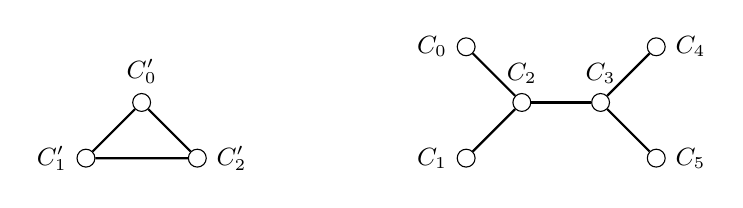
\begin{tikzpicture}
[node distance=1cm, font=\small]
\tikzstyle{vertex}=[circle, draw, fill=white, inner sep=0mm, minimum size=1.5ex]
\node[vertex]	(C2)  	at (1,0) [  label=above:{$C_2$}]{};
\node[vertex]	(C3)	[right of=C2,  label=above:{$C_3$}]{};
\node[vertex]	(C0)	[above left of=C2, label=left:{$C_0$}]{};
\node[vertex]	(C1)	[below left of=C2, label=left:{$C_1$}]{};
\node[vertex]	(C4)	[above right of=C3, label=right:{$C_4$}]{};
\node[vertex]	(C5)	[below right of=C3, label=right:{$C_5$}]{};

\node			(R)		[above left of =   C1, xshift=-1cm, label=below:{}]{};
\node			(R')	[above left of =   R,  xshift=-1cm, label=below:{}]{};

\node[vertex]	(C2')	[below left of = R, xshift=-1cm, label=right:{$C_2'$}]{};
\node[vertex]	(C0')	[above left of = C2', label=above:{$C_0'$}]{};
\node[vertex]	(C1')	[below left of = C0', label=left:{$C_1'$}]{};


\draw [thick] (C4)--(C3)--(C5);
\draw [thick] (C0)--(C2)--(C1);
\draw [thick] (C2)--(C3);

\draw[thick] (C0')--(C2')--(C1')--(C0');

\end{tikzpicture}
\end{gathered}
\end{equation*}
After renumeration, we may assume  that $(F\cdot C_0)=(F\cdot C'_0)=1$.
The   connected curve  $C_1+\ldots+C_5$ has dual graph $T_{2,2,3}$ and must be contained in   the fiber $\psi^{-1}(\infty)$.
Let $m\geq 2 $ be the multiplicity of $C_2\subset \psi^\inv_\ind(\infty)$.
From $2\geq \varphi^{-1}_\ind(\infty)\cdot \psi^{-1}(\infty)\geq C_0\cdot mC_2=m\geq 2$ we infer that the fiber $\psi^\inv(\infty)$
is simple. Likewise, $C'_1$ and $C'_2$ are $\psi$-vertical, say contained in $\psi_\ind^{-1}(0)$, with respective multiplicities $m_1,m_2\geq 1$.
Now
$$
2\geq \varphi^{-1}_\ind(\infty)\cdot \psi^{-1}(0)\geq C'_0\cdot (m_1C'_1+m_2C'_2) =m_1+m_2\geq 2,
$$
we see that  also $\psi^\inv(0)$ is simple, contradiction.
% and $m=2$, and hence its Kodaira symbol is $\I_n^*$.
% According to Proposition \ref{possible configurations},
% we have either $n=2$ or $n=4$.
% Now we use that the connected curve  $C'_1+C'_2$ is also contained in some fibers of $\psi$.
% 
% 
% For $n=2$ the configuration of fibers over rational points must be $\I_2^*+\III+\III$, which leaves no room
% for the $\psi$-vertical connected curve  $C'_1+C'_2$. 
% Thus $\psi^{-1}(\infty)$ has Kodaira symbol $\I_4^*$, consisting of the nine irreducible curves
% $C_1'+C_2'+ R'+R+C_1+\ldots+C_5$. The dual graph for our curves must take the following form:
% \begin{equation*}
% \begin{gathered}
% \begin{tikzpicture}
% [node distance=1cm, font=\small]
% \tikzstyle{vertex}=[circle, draw, fill=white, inner sep=0mm, minimum size=1.5ex]
% \node[vertex]	(C2)  	at (1,0) 	[ label=above:{$C_2$}]{};
% \node[vertex]	(C3)	[right of=C2,  label=above:{$C_3$}]{};
% \node[vertex]	(C0)	[above left of=C2, label=above:{$C_0$}]{};
% \node[vertex]	(C1)	[below left of=C2, label=below:{$C_1$}]{};
% \node[vertex]	(C4)	[above right of=C3, label=right:{$C_4$}]{};
% \node[vertex]	(C5)	[below right of=C3, label=right:{$C_5$}]{};
% 
% \node[vertex]	(R)	[above left of =   C1, xshift=-1cm, label=below:{$R$}]{};
% \node[vertex]	(R')	[above left of =   R,  xshift=-1cm, label=above:{$R'$}]{};
% 
% \node[vertex]	(C2')	[below left of = R, xshift=-1cm, label=below:{$C_2'$}]{};
% \node[vertex]	(C0')	[above left of = C2', label=  above left:{$C_0'$}]{};
% \node[vertex]	(C1')	[below left of = C0', label=below:{$C_1'$}]{};
% 
% 
% \draw [thick] (C4)--(C3)--(C5);
% \draw [thick] (C0)--(C2)--(C1);
% \draw [thick] (C2)--(C3);
% 
% \draw[thick] (C0')--(C2')--(C1')--(C0');
% \draw[thick] (C1)--(R)--(C2')--(R');
% \draw[dashed] (R)--(C0')--(R');
% \draw[dashed] (R)--(C0)--(R');
% \end{tikzpicture}
% \end{gathered}
% \end{equation*} 
% Recall that dashed edges represent potential intersections. However, we do not   have to analyse them further, because  
% $$
% 2=\varphi_\ind^\inv(0)\cdot \psi^\inv(\infty) = C'_0\cdot (C_1'+R' + 2C'_2 + 2R)\geq   (C'_0\cdot C_1') +  (C'_0\cdot 2C_2')=3
% $$
% already gives the desired  contradiction.
\qed

\medskip
Combining  Propositions  \ref{possible configurations} and \ref{no I8} and  \ref{no II*, IV*, IV}  we get the following key reduction:

\begin{proposition}
\source{no-enriques-surface-over-the-integers}
\notready
\mylabel{key reduction}
Suppose $Y$ is a non-exceptional Enriques surface over $k=\FF_2$ with constant Picard scheme.
Let $\varphi:Y\ra\PP^1$ be a genus-one fibration.
Up to  automorphisms of the projective line,
the possible configurations of fibers over the the rational points $t=0,1,\infty$ are given by
the following table:
$$
\begin{array}[c]{@{}lll}
\toprule
\text{elliptic}		& 		& \text{quasielliptic}\\
\midrule
\I_4^* +E_4+E_2		&		& \I_4^*+\II+\II\\
\midrule
\III^*+E_4+\I_2		&		& \III^*+\III+\II\\ 
\III^*+E_2+\tI_2\\
\III^*+E_4+E_4\\
\midrule
\I_1^*+E_4+\I_4	&		& \I_2^*+\III+\III\\
\bottomrule
\end{array}
$$
Moreover,   all $\I_1^*$-fibers are multiple, the fibers with Kodaira symbol  $\I_4^*,\I_n,\tI_2$ are simple,
and   there is another genus-one fibration
$\psi:Y\ra\PP^1$ with $\varphi^\inv(\infty)\cdot \psi^\inv(\infty)=4$.
\end{proposition}

% 
% %===========================================================
% \section{Elimination of \texorpdfstring{$\I_8$}{I8}-fibers}
% \mylabel{Elimination I8}
% 
% Let $Y$ be a non-exceptional Enriques surface over the ground field $k=\FF_2$,  with constant Picard scheme.
% The goal of this section is   to eliminate the last line from the table in Proposition \ref{key reduction}:
% 
% \begin{proposition}
% \mylabel{no I8}
% There is no genus-one fibration 
% $\varphi:Y\ra\PP^1$ having a fiber  with Kodaira symbol $\I_8$. 
% \end{proposition}
% 
% \proof
% Seeking a contradiction, we assume that $\varphi^{-1}(\infty)$ has Kodaira symbol $\I_8$. Then the fibration is elliptic, and
% the configuration
% of reducible fibers has dual graph:
% \begin{equation*}
% % dual graph I4*
% \begin{gathered}
% \begin{tikzpicture}
% [node distance=1cm, font=\small]
% \tikzstyle{vertex}=[circle, draw, fill=white, inner sep=0mm, minimum size=1.5ex]
% \node[vertex]	(C0)  	at (1,0) 	[label=above:{$C_0$}] 		{};
% \node[vertex]	(C1)			[below left of=C0, label=left:{$C_1$}]	{};
% \node[vertex]	(C2)			[below of=C1, label=left:{$C_2$}]	{};
% \node[vertex]	(C3)			[below right of=C2, label=below:{$C_3$}]	{};
% \node[vertex]	(C4)			[right of=C3, label=below:{$C_4$}]	{};
% \node[vertex]	(C5)			[above right of=C4, label=right:{$C_5$}]	{};
% \node[vertex]	(C6)			[above of=C5, label=right:{$C_6$}]	{};
% \node[vertex]	(C7)			[above left of=C6, label=above:{$C_7$}]	{};
%  
% \node[vertex]	(D0)			[above left of=C1, ,  xshift=-4em, yshift=-1em, label=above:{$D_0$}]	{};
% \node[vertex]	(D1)			[below left of=C2,  xshift=-4em, yshift=+1em, label=below:{$D_1$}]	{};
%  
% \draw[thick] (C0)--(C1)--(C2)--(C3)--(C4)--(C5)--(C6)--(C7)--(C0);
% \draw[thick,double] (D0)--(D1);
% \end{tikzpicture}
% \end{gathered}
% \end{equation*}
% \emph{Here the double edge indicates that the   scheme $D_0\cap D_1$ has length two}.
% The semistable fiber $\varphi^{-1}(\infty)$  is simple, hence reduced,
% whereas the fiber $\varphi^{-1}(0)$ with Kodaira symbol $\III$ is multiple.
% Moreover,  there is a genus-one fibration $\psi:Y\ra\PP^1$ so that the multiple fibers $2F$ have  
% $F\cdot \varphi^\inv_\ind(0)=1$. 
% After enumeration, we may assume   $(F\cdot D_1)=1$. So $D_0$ is vertical with respect to $\psi$,
% and we may assume that this is contained in 
% $\psi^\inv(\infty)=\sum_{i=0}^r m_iE_i$, say with $D_0=E_0$. Then
% $$
% 2\geq \psi^\inv_\ind(\infty)\cdot \varphi^\inv_\ind(0)=\sum_{i=0}^r m_i(E_i\cdot D_1)=2m_0 +\sum_{i=1}^r m_i(E_i\cdot D_1)\geq 2m_0.
% $$
% Hence the multiplicity is $m_0=1$,   the   fiber $\psi^\inv(\infty)$ is multiple, and    the curves $E_1,\ldots,E_r$ are disjoint from $D_1$.
% Furthermore, $r\geq 3$, because otherwise we get the contradiction $1=\psi^\inv_\ind(a)\cdot\varphi^\inv_\ind(0)=E_1\cdot D_0=2$.
% After renumeration, we may assume that $E_1$ is a neighbor of $E_0$ in the dual graph, such that $(E_1\cdot E_0)=1$. From
% $$
% 1=\psi^\inv_\ind(\infty)\cdot\varphi^\inv_\ind(0)= \sum_{i=1}^rm_iE_i\cdot (D_0+D_1) \geq m_1 (E_1\cdot D_0)=m_1
% $$
% we infer $m_1=1$. It follows that $\psi^\inv_\ind(\infty)$ is reduced.
% Summing up, $\psi^\inv_\ind(\infty)$ is multiple, reduced, and contains at least three irreducible components.
% According to Proposition \ref{key reduction}, this is impossible.
% \qed
% 

%===========================================================
